\section*{Úvod}
Tato zpráva se zabývá komplexním hodnocením vybraných kartografických zobrazení pomocí variačních kritérií s cílem posoudit jejich vhodnost pro znázornění rozsáhlých územních celků.
Jako zájmová oblast bylo pro účely této analýzy zvoleno území států bývalé Varšavské smlouvy.
Vzhledem k obrovské rozloze tohoto uskupení, které se táhlo od střední Evropy až po východní okraje Asie, je výběr optimálního mapového zobrazení klíčový pro minimalizaci nevyhnutelných zkreslení ploch, délek a úhlů. 

V rámci práce jsou analyzována zobrazení Bonneovo, Mercator-Sansonovo, Eckertovo V., Winkel-Tripel a Hammer-Aitoffovo.
K jejich kvantitativnímu zhodnocení je využito Airyho a komplexní variační kritérium, a to jak v základní, tak i ve vážené variantě.

Doplňujícím nástrojem pro vizuální posouzení kvality zobrazení je výpočet a vizualizace izočar měřítkového čísla mapy jakožto funkce polohy.
Veškeré potřebné výpočty, generování geografické sítě i závěrečné vizualizace byly provedeny vytvořeným skriptem v programovacím jazyce Python s využitím knihovny \lstinline|pyproj, matplotlib| a \lstinline|numpy|.

\newpage
\section*{Teorie ke zpracování}  
\subsection*{Variační kritéria } 

Pro hodnocení kartografických zobrazení se využívají složitější variační kritéria, jejichž cílem je zohlednit vliv délkového, úhlového a plošného zkreslení.
Tato kritéria umožňují komplexně zhodnotit vhodnost daného zobrazení pro konkrétní zájmové území.
Tento analytický přístup je důležitý zejména pro velké územní celky, u kterých nás zajímá nejen zkreslení na samotných okrajích, ale především celková věrnost zákresu vzdáleností, úhlů a ploch nad celým mapovým polem.
Pro takové případy jsou často preferována vyrovnávací zobrazení, jež sice zkreslují všechny tyto parametry, ale relativně málo. 
Jelikož běžné měřítko délek $m$ nabývá extrémních hodnot pouze u jednoduchých či konformních zobrazení, nejsou jeho hodnoty pro toto posouzení ideální.
Z toho důvodu představují vhodnější výchozí kvantitativní charakteristiku extrémní délková zkreslení, která jsou reprezentována poloosami $a$ a $b$ Tissotovy elipsy.

\subsubsection*{Lokální kritéria}
Poloosy $a$ a $b$ Tissotovy elipsy slouží jako základní vstupní parametry pro výpočet lokálních variačních kritérií v konkrétním bodě $P=[u,v]$. 
V rámci této práce jsou hodnocena následující dvě lokální kritéria:
\begin{itemize}
	\item \textbf{Airyho kritérium:} Zohledňuje primárně vliv délkového zkreslení, avšak nebere v potaz zkreslení úhlové. Je definováno vztahem:
	\begin{equation*}
	h^{2}(u,v)=\frac{1}{2}[(a-1)^{2}+(b-1)^{2}]
	\end{equation*}
	
	\item  \textbf{Komplexní kritérium:} 
	Toto kritérium přináší komplexnější pohled, jelikož díky zavedení členu $a/b$ kombinuje vliv délkového i úhlového zkreslení. Vypočte se jako:
	\begin{equation*}
	h^{2}(u,v)=\frac{1}{2}[|a-1|+|b-1|]+\frac{a}{b}-1 
	\end{equation*}
	
\end{itemize}  
  
\subsubsection*{Globální kritéria}
Abychom získali představu o deformaci nad celou zvolenou oblastí, určuje se tzv. globální variační kritérium $H^2$, které představuje střední hodnotu lokálního kritéria nad definovanou oblastí.
V praxi se pro výpočet u neortogonálních zobrazení využívá diskrétní varianta tohoto integrálu. 
Zájmové území se pokryje dostatečně hustou sítí uzlových bodů s pravidelnými rozestupy (kroky $\Delta u, \Delta v$).
V každém tomto uzlovém bodě se spočítají hodnoty lokálních kritérií $h^2(u,v)$ z poloos $a$ a $b$.
Výsledná hodnota globálního kritéria pak vzniká jako aritmetický nebo vážený průměr těchto lokálních hodnot.
Analýza se standardně provádí ve dvou variantách:
\begin{itemize}
	\item Nevážená varianta: Jedná se o prostý aritmetický průměr všech bodů:
	\begin{equation*}
		H_{1}^{2}=\frac{1}{n}\sum_{i=1}^{n}h^{2}(u_{i},v_{i}).
	\end{equation*}
	
	\item  Vážená varianta: Aby se potlačil vliv polárních oblastí na celkové hodnocení mapy, aplikuje se výpočet s váhou bodu $p_i$, která je funkcí zeměpisné šířky ($p_i = \cos u_i$). Vztah je definován jako:
	\begin{equation*}
		H_{2}^{2}=\frac{\sum_{i=1}^{n}p_{i}h^{2}(u_{i},v_{i})}{\sum_{i=1}^{n}p_{i}}.
	\end{equation*}
\end{itemize}
 

\subsection*{Měřítkové číslo} 
Kromě variačních kritérií se kvalita zobrazení hodnotí i vývojem měřítkového čísla $M(u,v)$ jakožto funkce polohy.
Měřítkové číslo v daném bodě je nepřímo úměrné maximálnímu délkovému zkreslení v tomto bodě, tedy hlavní poloose $a$ Tissotovy elipsy.
Vypočítá se podle vztahu $M(u,v) = \frac{M}{a(u,v)}$, kde $M$ představuje výchozí hodnotu měřítkového čísla (např. definovanou pro střed mapy a uvažovaný formát A4). 

 
\subsection*{Analyzovaná zobrazení}
\begin{itemize}
	\item \textbf{Bonneovo:} 
	Patří mezi nepravá kuželová zobrazení. Jedné se o zobrazení ekvivalentní. 
	Navíc je ekvidistantní podél nezkreslené rovnoběžky $u_0$ a podél všech ostatních rovnoběžek.
	Obrazem planisféry je charakteristický tvar srdce.
	\item \textbf{Mercartor-Sansonovo:}
	Jedná se o nepravé válcové zobrazení, konkrétně nepravé sinusoidální zobrazení.
	Je ekvivalentní a délkojevné v obrazu všech rovnoběžek a základního poledníku.
	Rovnoběžky jsou zobrazeny jako úsečky, poledníky jako sinusoidy.
	\item \textbf{Eckertovo V.:}
	Patří mezi nepravá válcová zobrazení.
	Jedná se o zobrazení vyrovnávací (kompenzační).
	Rovník a střední poledník jsou zobrazeny jako úsečky.
	Poledníky mají tvar sinusoid, rovnoběžky jsou zobrazeny jako úsečky.
	Póly zobrazeny jako úsečky o poloviční délce rovníku.
	\item \textbf{Winkel-Tripel:}
	Vyrovnávací modifikované azimutální zobrazení. 
	Vzniklo kombinací Aitoffova zobrazení a ekvidistantního válcového zobrazení.
	
	\item \textbf{Hammer-Aitoffovo:}
	Je modifikací Lambertova azimutálního ekvivalentního zobrazení.
	Jedná se tedy o ekvivalentní zobrazení.
	Střední poledník je úsečka o poloviční délce rovníku.
	Ostatní poledníky a rovnoběžky (kromě rovníku) jsou zobrazeny jako složité křivky.
\end{itemize}


\section*{Zpracování}
\subsection*{Vymezení území}
Jako zájmové území byly zvoleny státy Varšavské smlouvy. 
K vytvoření textového souboru se souřadnicemi bodů byly využity funkce v ArcGIS Pro.
Do SW byl nahrán shapefile polygonů se státy, ten byl poté převeden z polygonu na body, výsledné body byly exportovány do textového souboru.

Analyzované území byly ohraničeno okrajovými rovnoběžkami $u_1$ a $u_2$ a okrajovými poledníky $v_1$ a $v_2$:
\[ u_1 = 35^\circ, \qquad u_2 = 85^\circ, \qquad v_1 = 0^\circ, \qquad v_2 = 200^\circ.
\] 

Při vizualizaci zájmového území vyvstal specifický problém související s topologií geografických dat.
Území států bývalé Varšavské smlouvy totiž netvoří jeden spojitý polygon.
Kromě rozlehlé kontinentální pevninské masy zahrnuje také řadu geograficky oddělených celků, jako jsou například rozsáhlé sovětské ostrovy v Severním ledovém oceánu, nebo území států, která s hlavním blokem přímo nesousedila (např. Albánie).

Standardní vykreslovací funkce v knihovně \lstinline|matplotlib| (konkrétně funkce \lstinline|plot|) implicitně spojuje všechny načtené body ze souboru souvislou čarou.
Pokud datová sada obsahuje souřadnice více nespojitých polygonů uložených za sebou, algoritmus plynule přejde od posledního bodu jednoho celku k prvnímu bodu celku dalšího.
To vede ke vzniku nežádoucích křížících se čar napříč celým mapovým polem, jak ilustruje obrázek \ref{ob1}.

\begin{figure}[h!]
	\centering
	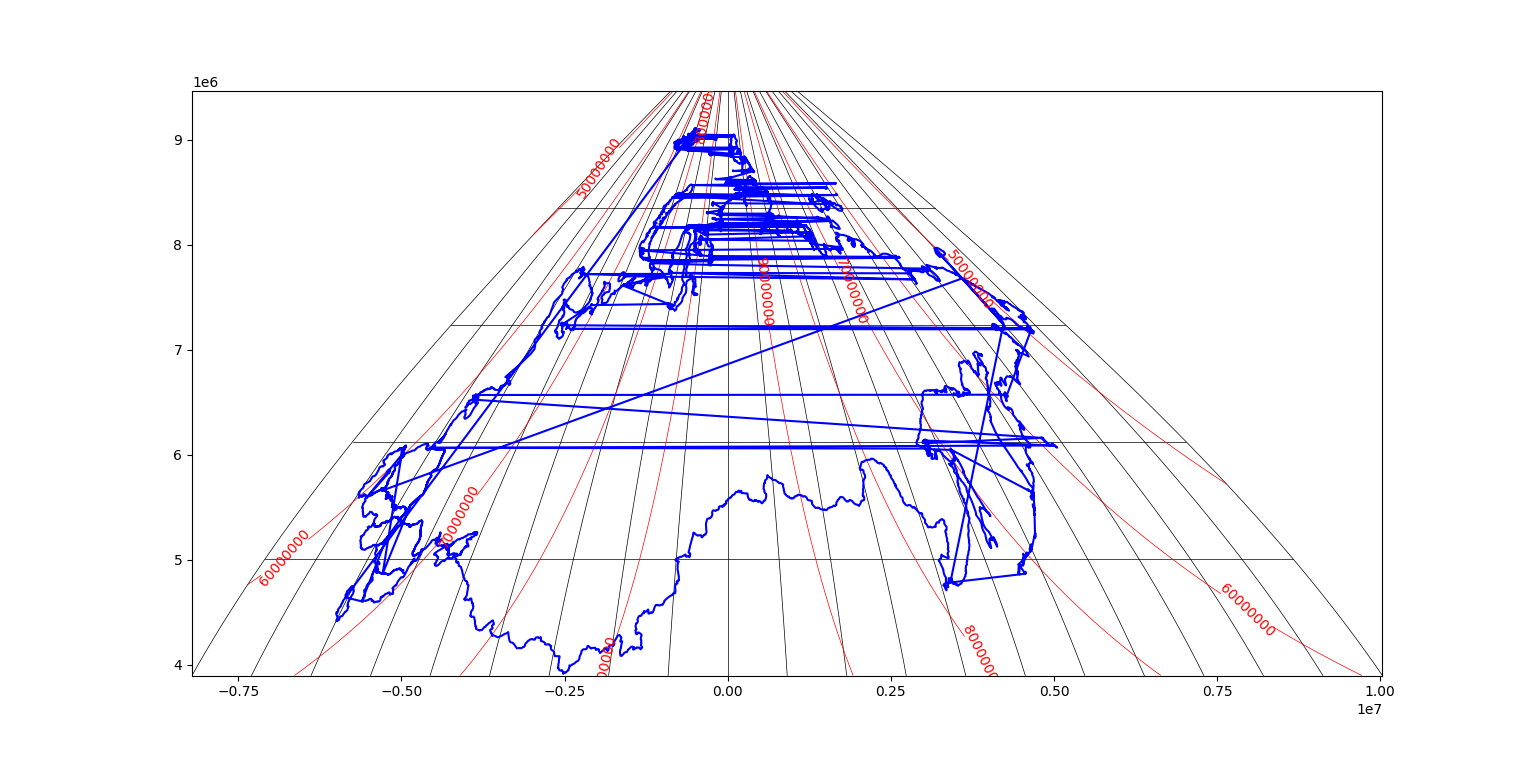
\includegraphics[width=1\linewidth]{figure/spatnevzkreslovani.png}
	\caption{Špatné vykreslení států.}
	\label{ob1}
\end{figure}

K eliminaci tohoto vizuálního defektu bylo nutné algoritmu říci, kde má takzvaně „zvednout pero“ a začít kreslit novou čáru.
K identifikaci těchto přechodů a celkovému vyřešení problému byl s využitím nástrojů umělé inteligence implementován doplňující algoritmus (viz kód níže).

Jeho princip spočívá v analytickém výpočtu vzdálenosti mezi všemi po sobě jdoucími body.
Pokud vypočtená vzdálenost přesáhne stanovenou hranici (v tomto případě vzdálenost větší než 2 stupně), program tento úsek detekuje jako nepřirozený skok mezi dvěma oddělenými územími.
Na příslušný index je následně vložena nedefinovaná hodnota NaN.
Vykreslovací funkce při narazení na hodnotu NaN čáru přeruší a plynule pokračuje ve vykreslování až od následujících validních souřadnic, čímž je zaručeno korektní zobrazení členitých hranic.

\begin{lstlisting}[language=Python, caption = Vyřešní problému s vykreslováním.]
#Calculate the distance between every consecutive point
distances = np.sqrt(np.sum(np.diff(continents, axis=0)**2, axis=1))

#Find where the distance jumps by an unnaturally large amount (e.g., > 2 degrees)
jump_indices = np.where(distances > 2.0)[0] + 1

#Insert NaN values at those jump locations to "lift the pen"
continents = np.insert(continents, jump_indices, np.nan, axis=0)
\end{lstlisting}

\section*{Výsledky}
\subsection*{Variační kritéria}
V rámci kvantitativního hodnocení analyzovaných kartografických zobrazení byly pro zvolené území států bývalé Varšavské smlouvy vypočteny hodnoty globálních variačních kritérií. 
Pro posouzení deformací bylo využito jak Airyho kritérium (zohledňující primárně délkové zkreslení), tak i komplexní kritérium (kombinující vliv délkového a úhlového zkreslení). 
Aby se minimalizoval vliv extrémních zkreslení v odlehlejších (zejména polárních) oblastech, které by mohly celkové hodnocení mapy negativně ovlivnit, byly u obou kritérií vedle základních (nevážených) variant vypočteny také varianty vážené.
Kompletní výsledky těchto výpočtů přehledně shrnuje tabulka \ref{tab1}. 


Z naměřených hodnot je patrné, že aplikace vážené varianty u všech zkoumaných zobrazení skutečně vede k nižším hodnotám globálního zkreslení.
Z tabulky rovněž jasně vyplývá, že suverénně nejnižších hodnot u obou sledovaných kritérií dosahuje Bonneovo zobrazení (např. vážené Airyho kritérium nabývá hodnoty pouhých $0,00566$).
Naopak nejméně vhodnými pro tento specifický územní celek se jeví Eckertovo V. zobrazení, které vykazuje extrémní hodnoty u neváženého Airyho kritéria, a zobrazení Mercator-Sansonovo, jež dosahuje nejvyšších deformací v rámci komplexního kritéria.


\begin{table}[h!]
	\centering
	\begin{tabular}{|c||c|c|c|c|}
		\hline
		& \multicolumn{2}{c|}{Airyho kritérium} & \multicolumn{2}{c|}{Komplexní kritérium} \\
		\hline
		& nevážená var. & vážená var. & nevážená var. & vážená var. \\
		\hline \hline
		Bonneovo z. & 0,01001 & 0,00566 & 0,22626 & 0,17050 \\
		\hline
		Mercator-Sansonovo z. & 0,20677 & 0,17947 & 1,60622 & 1,46692 \\
		\hline
		Eckertovo V. z. & 0,75022 & 0,26829 & 1,59169 & 1,04196 \\
		\hline
		Winkel-Tripel z. & 0,34825 & 0,12828 & 1,00637 & 0,66856 \\
		\hline
		Hammer-Aitoffovo z. & 0,21384 & 0,15430 & 1,26317 & 1,06225 \\
		\hline
	\end{tabular}
	\caption{Výsledné hodnoty variačních kritérií pro zadaná zobrazení.}
	\label{tab1}
\end{table}

\newpage
\subsection*{Izočáry měřítkového čísla}
Doplňujícím nástrojem pro hodnocení kvality a distribuce zkreslení v mapovém poli je vizualizace izočar měřítkového čísla $M(u,v)$. 
Zatímco variační kritéria poskytují jediné souhrnné číslo pro celé území, izočáry umožňují prostorovou analýzu toho, jak se měřítko mapy mění v závislosti na poloze. 

\textbf{Metodika výpočtu:}
V každém bodě výpočetní sítě bylo měřítkové číslo stanoveno jako funkce polohy podle vztahu: $$M(u,v) = \frac{M}{a(u,v)}$$ kde $M$ představuje výchozí měřítko mapy a $a(u,v)$ je délka hlavní poloosy Tissotovy indikatrix, která reprezentuje maximální délkové zkreslení v daném bodě. 
Pro účely vizualizace bylo zvoleno základní měřítko $M = 100\,000\,000$ (odpovídající přehledné mapě daného celku) a izočáry byly generovány v konstantním kroku $10\,000\,000$.

\begin{itemize}
\item \textbf{Bonneovo zobrazení:} Vykazuje nejstabilnější průběh měřítkového čísla nad většinou zájmového území.
Izočáry mají charakteristický tvar vycházející z nezkreslené rovnoběžky.

\item \textbf{Mercator-Sansonovo zobrazení:} Izočáry sledují sinusoidální průběh poledníků.
Se zvyšující se zeměpisnou šířkou a vzdáleností od základního poledníku dochází k prudšímu poklesu měřítkového čísla (nárůstu zkreslení).

\item \textbf{Winkel-Tripel a Hammer-Aitoffovo zobrazení:} Jakožto vyrovnávací zobrazení vykazují plynulejší přechody mezi hodnotami.
Izočáry jsou u těchto zobrazení více rozestoupené, což indikuje pozvolnější změnu měřítka, což je pro mapy velkých celků žádoucí vlastnost.

\item \textbf{Eckertovo V. zobrazení:} Zde je patrný vliv lineárních pólů, kdy izočáry měřítkového čísla vykazují výrazné zahuštění směrem k okrajům a vyšším šířkám, což potvrzuje vyšší hodnoty variačních kritérií zjištěné v předchozí kapitole.
\end{itemize}

\begin{figure}[H]
	\centering
	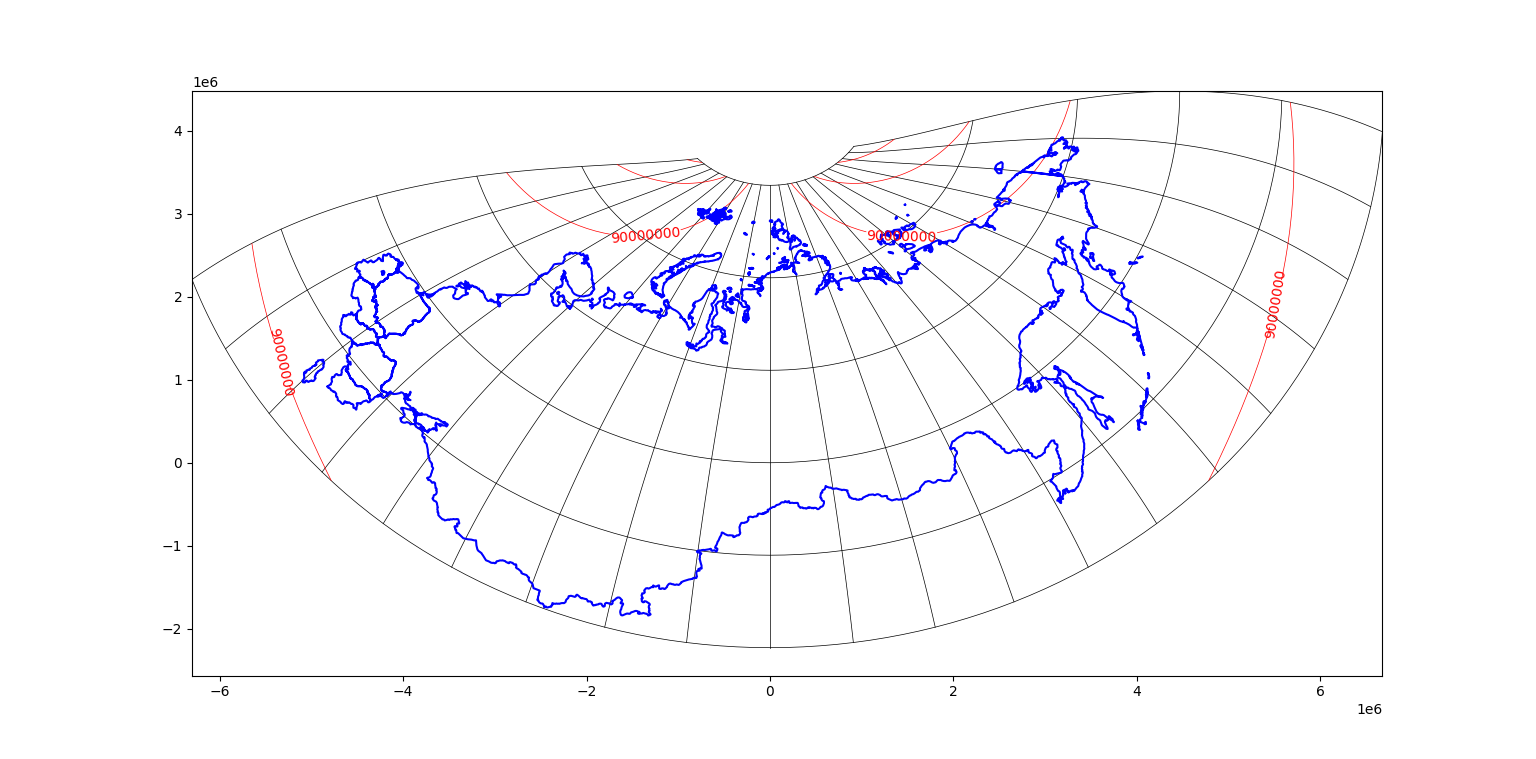
\includegraphics[width=1\linewidth]{figure/bonne.png}
	\caption{Bonneovo zobrazení.}
	\label{ob2}
\end{figure}


\begin{figure}[H]
	\centering
	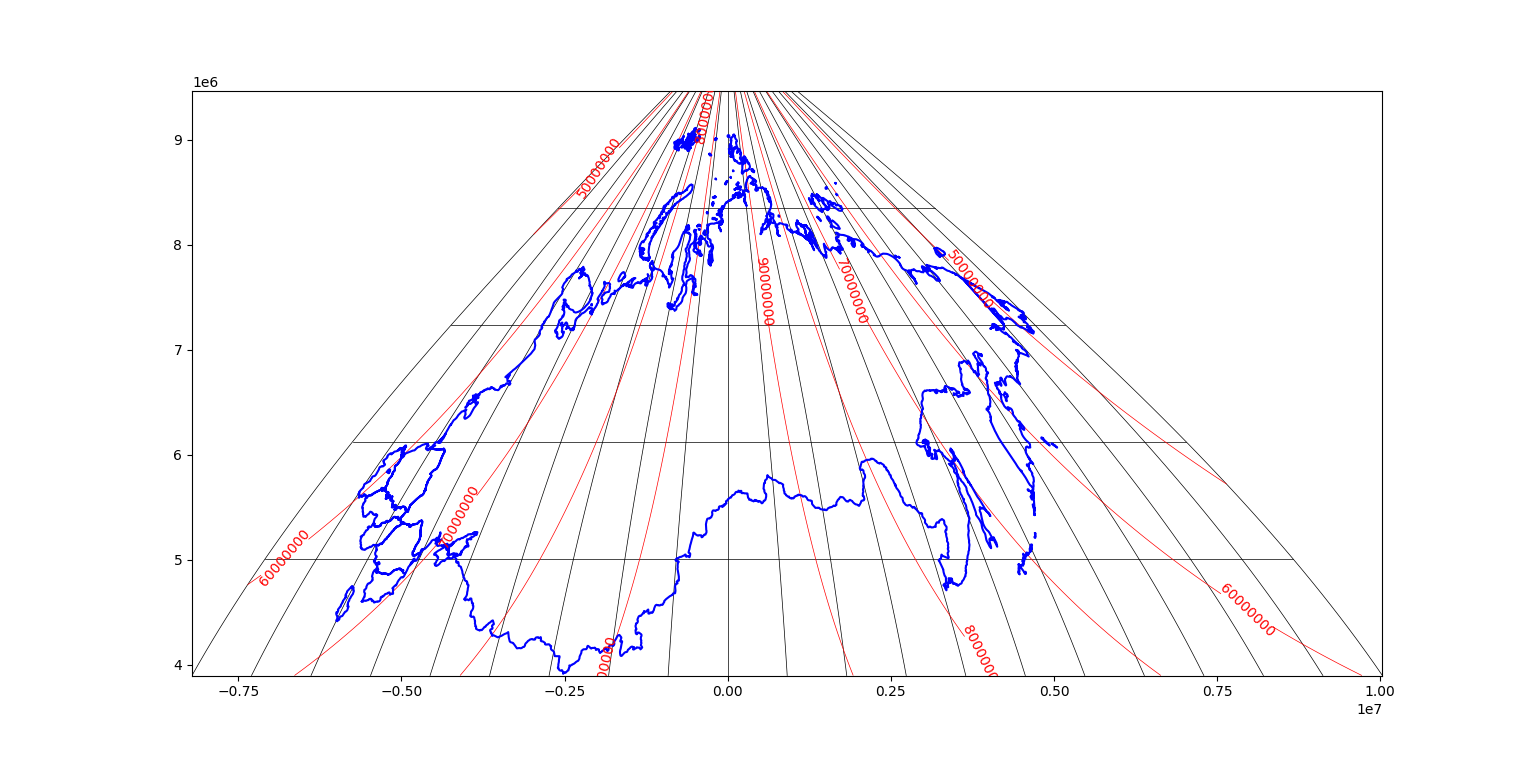
\includegraphics[width=1\linewidth]{figure/sinu.png}
	\caption{Mercartor-Sansonovo zobrazení.}
	\label{ob3}
\end{figure}

\begin{figure}[H]
	\centering
	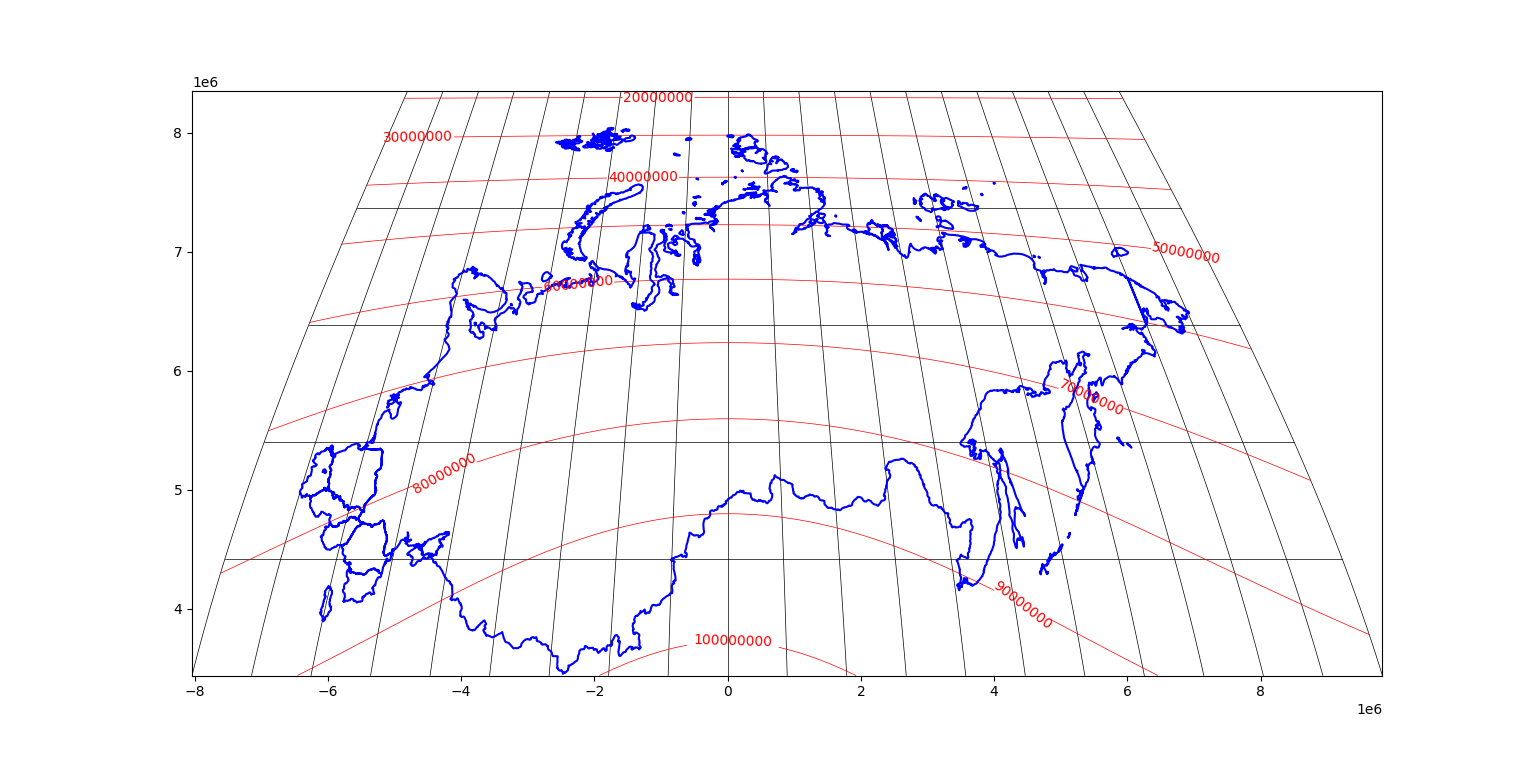
\includegraphics[width=1\linewidth]{figure/eck5.png}
	\caption{Eckertovo V. zobrazení.}
	\label{ob4}
\end{figure}


\begin{figure}[H]
	\centering
	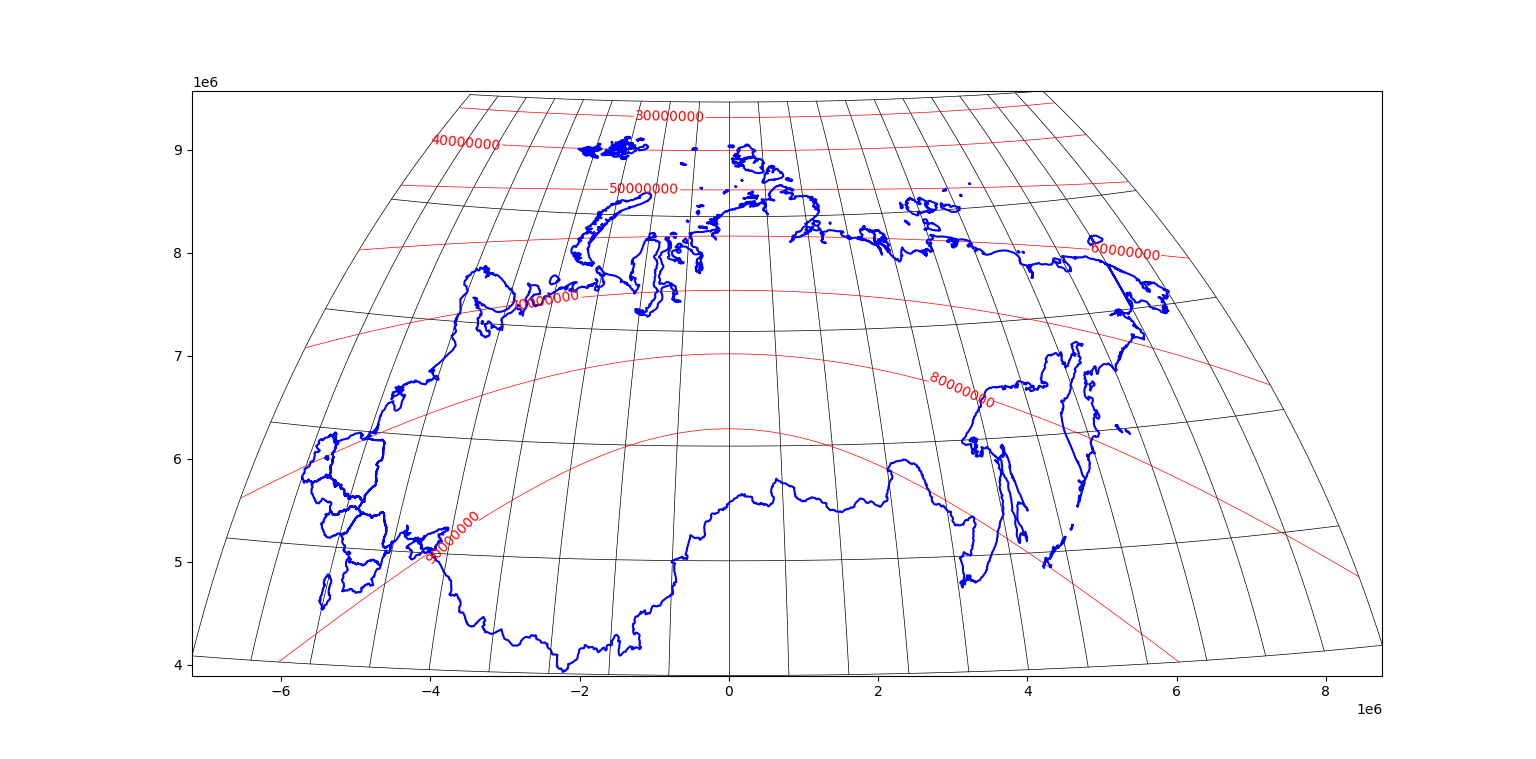
\includegraphics[width=1\linewidth]{figure/wintriple.png}
	\caption{Winkel-Tripel zobrazení.}
	\label{ob5}
\end{figure}


\begin{figure}[H]
	\centering
	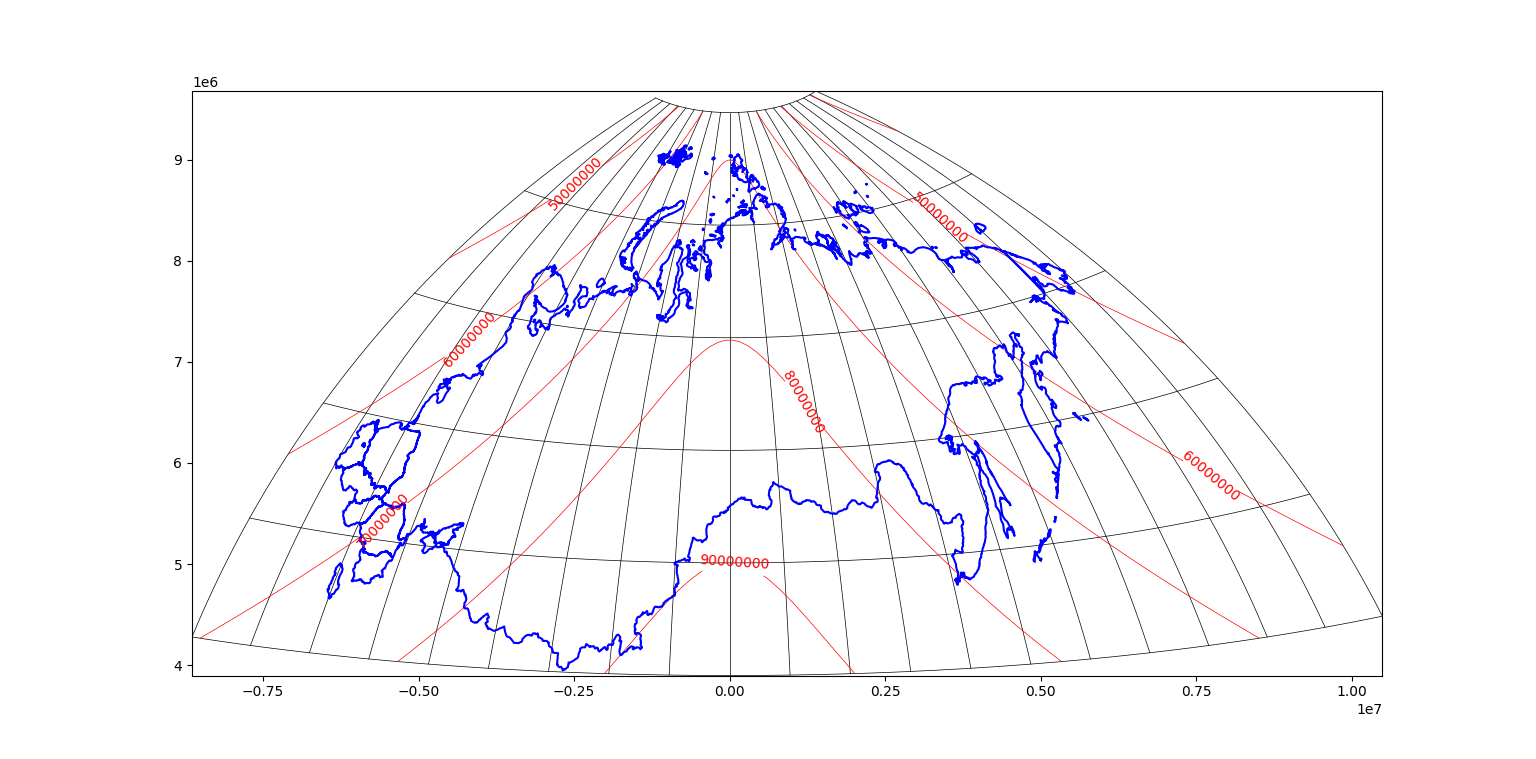
\includegraphics[width=1\linewidth]{figure/Aitoff.png}
	\caption{Hammer-Aitoffovo zobrazení.}
	\label{ob6}
\end{figure}

\newpage
\subsection*{Plošná analýza změn měřítkového čísla}
V rámci detailnějšího posouzení vhodnosti jednotlivých zobrazení byla provedena plošná analýza deformací měřítka.
Cílem bylo kvantifikovat, jak velká část zájmového území vykazuje relativní změnu měřítkového čísla menší než 50~\% oproti jeho výchozí hodnotě (matematicky vyjádřeno jako podmínka $|1/a - 1| < 0,5$).
Vzhledem k faktu, že se poledníky směrem k pólům sbíhají a plošný obsah sférických lichoběžníků klesá, nelze podíl území počítat prostým poměrem počtu uzlových bodů.
Výpočet byl proto realizován pomocí váženého součtu, kde váha každého uzlového bodu odpovídá kosinu jeho zeměpisné šířky ($p_i = \cos u_i$).
Jak ukazují výsledky, nejstabilnějším se v tomto ohledu ukázalo být Bonneovo zobrazení, u kterého se změna měřítkového čísla udržela pod hranicí 50~\% na plných 100~\% celkové plochy zájmového území.
Naopak největším výkyvům čelí zobrazení Eckertovo V., kde tuto toleranci splňovalo pouze 90,42~\% území, což plně koresponduje s průběhem izočar analyzovaných v předchozí podkapitole a potvrzuje jeho nevhodnost pro takto prostorově rozsáhlý celek.
Tabulka~\ref{tab2} zobrazuje výsledky pro všechna zobrazení.


\begin{table}[H]
	\centering
	\begin{tabular}{|c||c|}
		\hline
		Zobrazení & Procento území, kde změna M < 50 \% \\
		\hline \hline
		Bonneovo  & 100 \%  \\
		\hline
		Mercator-Sansonovo  & 96.41 \%  \\
		\hline
		Eckertovo V.  & 90.42 \%  \\
		\hline
		Winkel-Tripel  & 94.66 \% \\
		\hline
		Hammer-Aitoffovo  & 95.32 \% \\
		\hline
	\end{tabular}
	\caption{Výsledky analýzy změny měřítkového čísla.}
	\label{tab2}
\end{table}

\newpage
\section*{Závěr a hodnocení}
Na základě provedených výpočtů globálních variačních kritérií lze jednoznačně konstatovat, že nejvhodnějším kartografickým zobrazením pro znázornění území států bývalé Varšavské smlouvy je Bonneovo zobrazení.
Toto zobrazení dosahuje nejnižších hodnot zkreslení napříč všemi testovanými metrikami.
Ve vážené variantě Airyho kritéria klesla hodnota na pouhých 0,00566 a u komplexního kritéria na 0,17050.
Pro území, které je takto masivně protažené v rovnoběžkovém směru a nachází se převážně ve středních a vyšších zeměpisných šířkách, se toto ekvivalentní zobrazení jeví jako ideální volba.
Jako druhé v pořadí se s relativně přijatelnými hodnotami umístilo zobrazení Hammer-Aitoffovo. 
Naopak jako zcela nevhodná pro tento konkrétní územní celek se ukázala zobrazení Eckertovo V. a Mercator-Sansonovo.
Eckertovo zobrazení vykazuje enormní nárůst u Airyho kritéria (0,75022 v nevážené variantě), což značí extrémní délkové deformace.
Mercator-Sansonovo zobrazení pak naprosto selhává u komplexního kritéria (1,60622), což ukazuje na masivní úhlová zkreslení v okrajových částech zkoumaného území.
Tyto numerické závěry plně korespondují s vizuální analýzou izočar měřítkového čísla.
U Bonneova zobrazení se měřítko v závislosti na poloze mění nejpomaleji a izočáry jsou stabilní nad drtivou většinou zájmové oblasti.
U ostatních zobrazení (zejména Eckert V.) dochází k prudkým skokům a zahušťování izočar směrem k pólům.

Z hlediska hodnocení samotných variačních kritérií se jako objektivnější a více vypovídající nástroj jeví komplexní kritérium.
Airyho kritérium zohledňuje primárně vliv délkového zkreslení a úhlové deformace prakticky ignoruje.
Naproti tomu komplexní kritérium vhodně kombinuje vliv délkového i úhlového zkreslení současně.
Pro mapu takto obrovského územního celku, kde může docházet k silnému zkreslení úhlů, je právě tento kombinovaný přístup zásadní.
Pro úplnou a správnou interpretaci vlastností mapy je však vždy nejlepší cestou kombinovat obě tyto analytické metody - jak numerický výpočet globálních kritérií, tak i názornou prostorovou vizualizaci pomocí izočar měřítkového čísla. 